\chapter{Detalii de implementare}
\section{Detaliile modulului front-end}
Modulul \textit{front-end} este realizat cu ajutorul \textit{framework}-ului Angulare, folosind limbajul Typescript și tehnologiile HTML și CSS.

Este împărțit în 3 componente: \textit{HomeComponent}, \textit{LoginComponent} și \textit{ImageUploadComponent} și folosește 3 servicii: \textit{AuthService}, \textit{Auth-GuardService} și \textit{ImageService}.

\subsection{HomeComponent}
 Se află pe ruta /home și este prima componentă cu care interacționează orice utilizatorul. Rolul ei este de a oferi informații despre aplicație și a facilita procesul de logare. Are un singur buton, cel de "Login", care atunci când este apăsat va redirecta utilizatorul spre modulul de \textit{back-end} pentru continuarea procesului de logare.
 
 \subsection{LoginComponent}
 Această componentă are ruta /login/:id, unde parametrul id va reprezenta identificatorul utilizatorului trimis de către serviciul de \textit{back-end} prin redirectare. În cadrul componentei se va prelua valoarea parametrului din rută și se va apela funcția login din cadrul serviciului \textit{AuthService}. Această funcție se ocupă de salvarea identificatorului. Inițial acesta era salvat în LocalStorage, dar din considerente de securitate, s-a ales ca soluție SessionStorage, care se golește la părăsirea sesiunii curente. Componenta apelează din nou \textit{AuthService} și pentru a cere modulului de \textit{back-end} informații despre profilul de Flickr ale utilizatorului, informații salvate în cadrul serviciului. După aceste acțiuni, se folosește routerul din Angular pentru a redirecta utilizatorul către următoarea componentă, \textit{ImageUploadComponent}.
 
 \subsection{ImageUploadComponent}
Componenta aferentă rutei /upload, care este o rută protejată prin o gardă de rută. Gărzile de rută în Angular sunt interfețe care îi spun routerului dacă poate sau nu naviga la o anumită rută. Routerul decide în funcție de o valoare booleană returnată de o clasă care implementează interfața gărzii. În cadrul aplicației s-a folosit garda CanActivate, a cărei interfață a fost implementată de serviciul Auth-GuardService. Acesta conține o metodă care returnează valoarea adevărat pentru când utilizatorul este autentificat ( se determină cu ajutorul metodei isAuthenticated din cadrul AuthService, care caută dacă este salvat vreun identificator în SessionStorage) și fals pentru cazul în care nu este autentificat. Astfel ImageUploadComponent este accesibilă doar unui utilizator autentificat.

Componenta conține un buton "Choose Files" care odată apăsat deschide o fereastră de unde utilizatorul va alege o imagine, butonul având în spate un \textit{input} HTML de tip imagine. După ce utilizatorul selectează o imagine, se va apela funcția \textit{preview}, care va citi conținutul imaginii și o va afișa pe ecran, pentru ca utilizatorul să își vizualizeze selecția.În cadrul paginii există și un grup de 3 \textit{radio-buttons}, care permit utilizatorului să selecteze de unde vrea să provină imaginile care vor fi analizate pentru a determina similaritatea. Opțiunile sunt profilul de Flickr utilizatorului, imaginile utilizatorilor din lista sa de contacte sau imaginile publice de pe Flickr, în mod implicit fiind selectată opțiunea corespunzătoare propriului profil.

Apăsarea butonului de "Upload" va apela funcția cu același nume. Funcția va afișa un element de tip \textit{spinner} pe ecran pentru a indica utilizatorului procesarea cererii. De asemenea va prelua identificatorul cu ajutorul funcției getUser din AuthService, funcție ce preia identificatorul din SessionStorage. Componenta va apela funcția postImage din serviciul ImageService, folosind imaginea în format base64,  identificatorul utilizatorului și opțiunea acestuia ca parametrii.

Folosind clientul de http din Angular, ImageService transmite o cerere la \textit{back-end} și returnează răspunsul acestuia. În funcție de răspuns, componenta va afișa lista de etichete aferente imaginii și imaginile similare vizual, sau un mesaj explicativ în cazul în care nu au fost găsite etichete/imagini.

\section{Detaliile modulului back-end}
\subsubsection{Autentificarea cu OAuth}
Pentru a realiza autentificarea pe platforma Flickr prin protocolul OAuth, aplicația folosește o bibliotecă de cod numită \textit{AuthLib} ce furnizează un client OAuth pentru Flask. Clientul este înregistrat în aplicație folosind anumite configurări (id-ul clientului, url-ul pentru autorizare, etc.) dintr-un fișier de configurări. Atunci când este accesată ruta /login, aplicația primește prin intermediul clientului OAuth un \textit{request token} și generează un identificator unic pentru utilizatorul ce a accesat ruta, salvând \textit{token}-ul într-un sistem de cache, apoi redirectează către ruta /authorize.

În cadrul funcției ce gestioneaza ruta /authorize, clientul OAuth schimbă \textit{request token}-ul, cu un \textit{token} OAuth de acces, pe care aplicația îl va salva împreună cu identificatorul generat într-o bază de date, apoi utilizatorul va fi redirectat la modulul de \textit{front-end}.

\subsection{Informații despre profil}
Aplicația va face o cerere la una din metodele disponibile prin API-ul Flickr, va împacheta informațiile cerute(nume utilizator și imagine de profil) într-un JSON și le va returna.

\subsection{Analiza unei imagini}
Pentru analiza unei imagini se folosește un model de rețea neurală disponibil prin biblioteca Keras. Numit \textit{NASNEtMobile} acest model este alcătuit din mai multe straturi convoluționale, fiind o versiune scalată a arhitecturii \textit{NASNet}, versiune optimizată pentru viteză crescută. Modelul este preantrenat pe setul de date ImageNet, putând clasifica imagini în 1000 categorii.
Biblioteca Keras oferă mai multe modele de rețele neurale preantrenate pe același set de date, figura ~\ref{fig:networks} conținând specificațiile lor.

\begin{figure}[!htbp]
    \begin{center}
        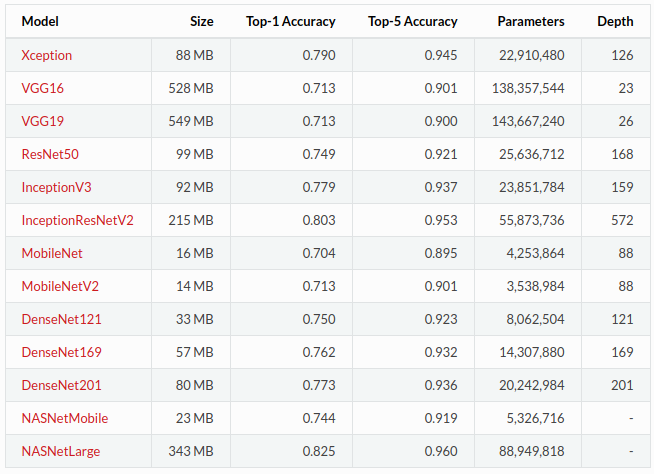
\includegraphics[width=0.8\textwidth]{images/neuralnetworks.png}
        \caption{Modelele de rețele disponibile prin Keras\label{fig:networks}}
    \end{center}
\end{figure}

Pentru a alege un anume model, s-au testat mai multe din cele disponibile, apoi s-a încercat a se face un compromis între acuratețe și viteza de analiză a unei imagini (cunoscută ca și viteza de \textit{forward-pass} în rețea). Ambii parametrii depind de mărimea modelului, numărul de parametrii, tipul de straturi folosite, precum și arhitectura modelului în general.

De asemenea viteza depinde și de mărimea imaginii analizate(aceeași indiferent de model) și mărimea la care trebuie dimensionată imaginea pentru a fi acceptată de model(diferită). În tabela \ref{table:1} se găsesc comparații ale modelelor încercate ținând cont de viteza medie de analiza a unei imagini (prima imagine după instanțierea modelului durează mai mult și nu a fost luată în considerare pentru medie), acuratețea modelului și mărimea datelor de intrare acceptate( în format (lățime, înălțime) ).


\begin{table}[h!]
\centering
 \begin{tabular}{||c c c c c||} 
 \hline
 Model & Viteză medie & Acuratețe top-1 & Acuratețe top-5 & Format \\ [0.5ex] 
 \hline\hline
 NASNetMobile & 0.25 secunde & 0.7444 & 0.919 &(224,224) \\ 
 \hline
 ResNet50 & 0.6 secunde & 0.749 & 0.921 & (224,224) \\
 \hline
 MobileNetV2 & 0.25 secunde & 0.713 & 0.901 & (224,224) \\
 \hline
 VGG16 & 0.5 secunde & 0.713 & 0.901 & (224,224)  \\
 \hline
 InceptionResNetV2 & 1.23 secunde & 788 & 6344 &  (299,299) \\ [1ex] 
 \hline
\end{tabular}
\caption{Comparație între modelele încercate}
\label{table:1}
\end{table}

Fiecare model acceptă propriul tip de date de intrare, din acest motiv trebuie folosite funcțiile de preprocesare corespunzătoare, disponibile împreună cu modelul în biblioteca Keras. Modelul returnează o listă de predicții ce trebuie interpretată folosind din nou o funcție specifică modelului. După aceasta se obține  o listă de tuple, primul element din tuplă fiind o eticheta ce  descrie imaginea, iar al doilea fiind probabilitatea etichetei de a descrie corect imaginea.

Instanțierea modelului, preprocesarea imaginii și obținerea predicțiilor se realizează în modul următor:

 
\definecolor{codegreen}{rgb}{0,0.6,0}
\definecolor{codegray}{rgb}{0.5,0.5,0.5}
\definecolor{codepurple}{rgb}{0.58,0,0.82}
\definecolor{backcolour}{rgb}{0.95,0.95,0.92}
 
\lstdefinestyle{mystyle}{
    backgroundcolor=\color{backcolour},   
    commentstyle=\color{codegreen},
    keywordstyle=\color{magenta},
    numberstyle=\tiny\color{codegray},
    stringstyle=\color{codepurple},
    basicstyle=\footnotesize,
    breakatwhitespace=false,         
    breaklines=true,                 
    captionpos=b,                    
    keepspaces=true,                 
    numbers=left,                    
    numbersep=5pt,                  
    showspaces=false,                
    showstringspaces=false,
    showtabs=false,                  
    tabsize=2
}
 
\lstset{style=mystyle}

\begin{lstlisting}[language=Python]
# obtinerea modelului preantrenat
model = NASNetMobile(weights="imagenet")
# decodarea imaginii din base64
image_response = base64.b64decode(image_response)
# citirea continutului imaginii
img = image.load_img(BytesIO(image_response), target_size=(224, 224))
# procesarea imaginii in numpy
img = image.img_to_array(img)
img = np.expand_dims(img, axis=0)
# preprocesarea conform specificatiilor modelului
img = preprocess_input(img)
# obtinerea predictiilor
predictions = model.predict(img)
#decodificarea predictiilor
predictions = decode_predictions(predictions)[0]
\end{lstlisting}

În funcție de cerințe, aplicația folosește și un parametru care precizează probabilitatea minimă acceptată pentru o etichetă ca aceasta să se regăsească în lista de etichete finală, acest parametru având momentan valoarea de 0.25.

\subsection{Aducerea imaginilor de pe Flickr}